\documentclass[]{article}

\usepackage{parskip,amsmath,graphicx}
\usepackage[margin=0.5in]{geometry}
\usepackage[section]{placeins}
\usepackage{pdfpages,bm}

%opening
\title{Final Project - ASE 389P.8 Satellite Control Systems}
\author{Corey Marcus}

\begin{document}

\maketitle

\newcommand{\CrossProd}[1]{\left[ #1 \times \right]}

\section{Introduction}

An eccentric billionaire has built his own space station. To save on design costs, his station is an exact replica of the ISS. He does not intend to share it with anyone, so it was scaled down in size such that its inertia matrix is smaller than that of the ISS by a factor of 1E-4. However, he demanded the station be as fast and nimble as his companies (he is a disruptor). The station's CMGs have the performance as the full size ISS. Super cooled bearings made of unobtainium mean there is no limit on how fast the gimbals can spin. 

\section{Attitude Dynamics and Kinematics}

The station lives in an equatorial 400km circular orbit. Its attitude is perturbed by gravity gradient. The angular inertia matrix is given by
\begin{equation}
	\bm{J} = 10^{-4} \begin{bmatrix}
		24181836 & 3783405 & 3898808 \\
		3783405 & 37621803 & -1171849 \\
		3898808 & -1171849 & 51576634
	\end{bmatrix}
\end{equation}

\section{Reference Attitude}

The station is generally prescribed to remain fixed with respect to the LVLH frame. It begins with a nominal quaternion $\begin{bmatrix} 0.028 & -0.0788 & 0.1141 & 0.9899 \end{bmatrix} $ from LVLH to body and angular rate with respect to the LVLH frame of zero. Through the course of a 100 run Monte Carlo (MC), the nominal quaternion and angular rate are dispersed using zero-mean gaussian noise with covariance $10^{-2}\bm{I}_{3 \times 3}$ and $10^{-3}\bm{I}_{3 \times 3}$.

The station is commanded to rotate to quaternion $\begin{bmatrix} 0.0481 & -0.0500 & 0.1420 & 0.9874 \end{bmatrix} $  with respect to the LVLH frame and then remain fixed. This corresponds to a 3 degree rotation about each body axis. The reference rotation is designed as a constant angular rate euler-axis rotation.

Figures \ref{fig:MC_quat_command_perf.pdf} and \ref{fig:MC_rate_command_perf.pdf} show the estimated command errors, or difference between the estimated pose and desired pose.

\begin{figure}[!h]
	\centering
	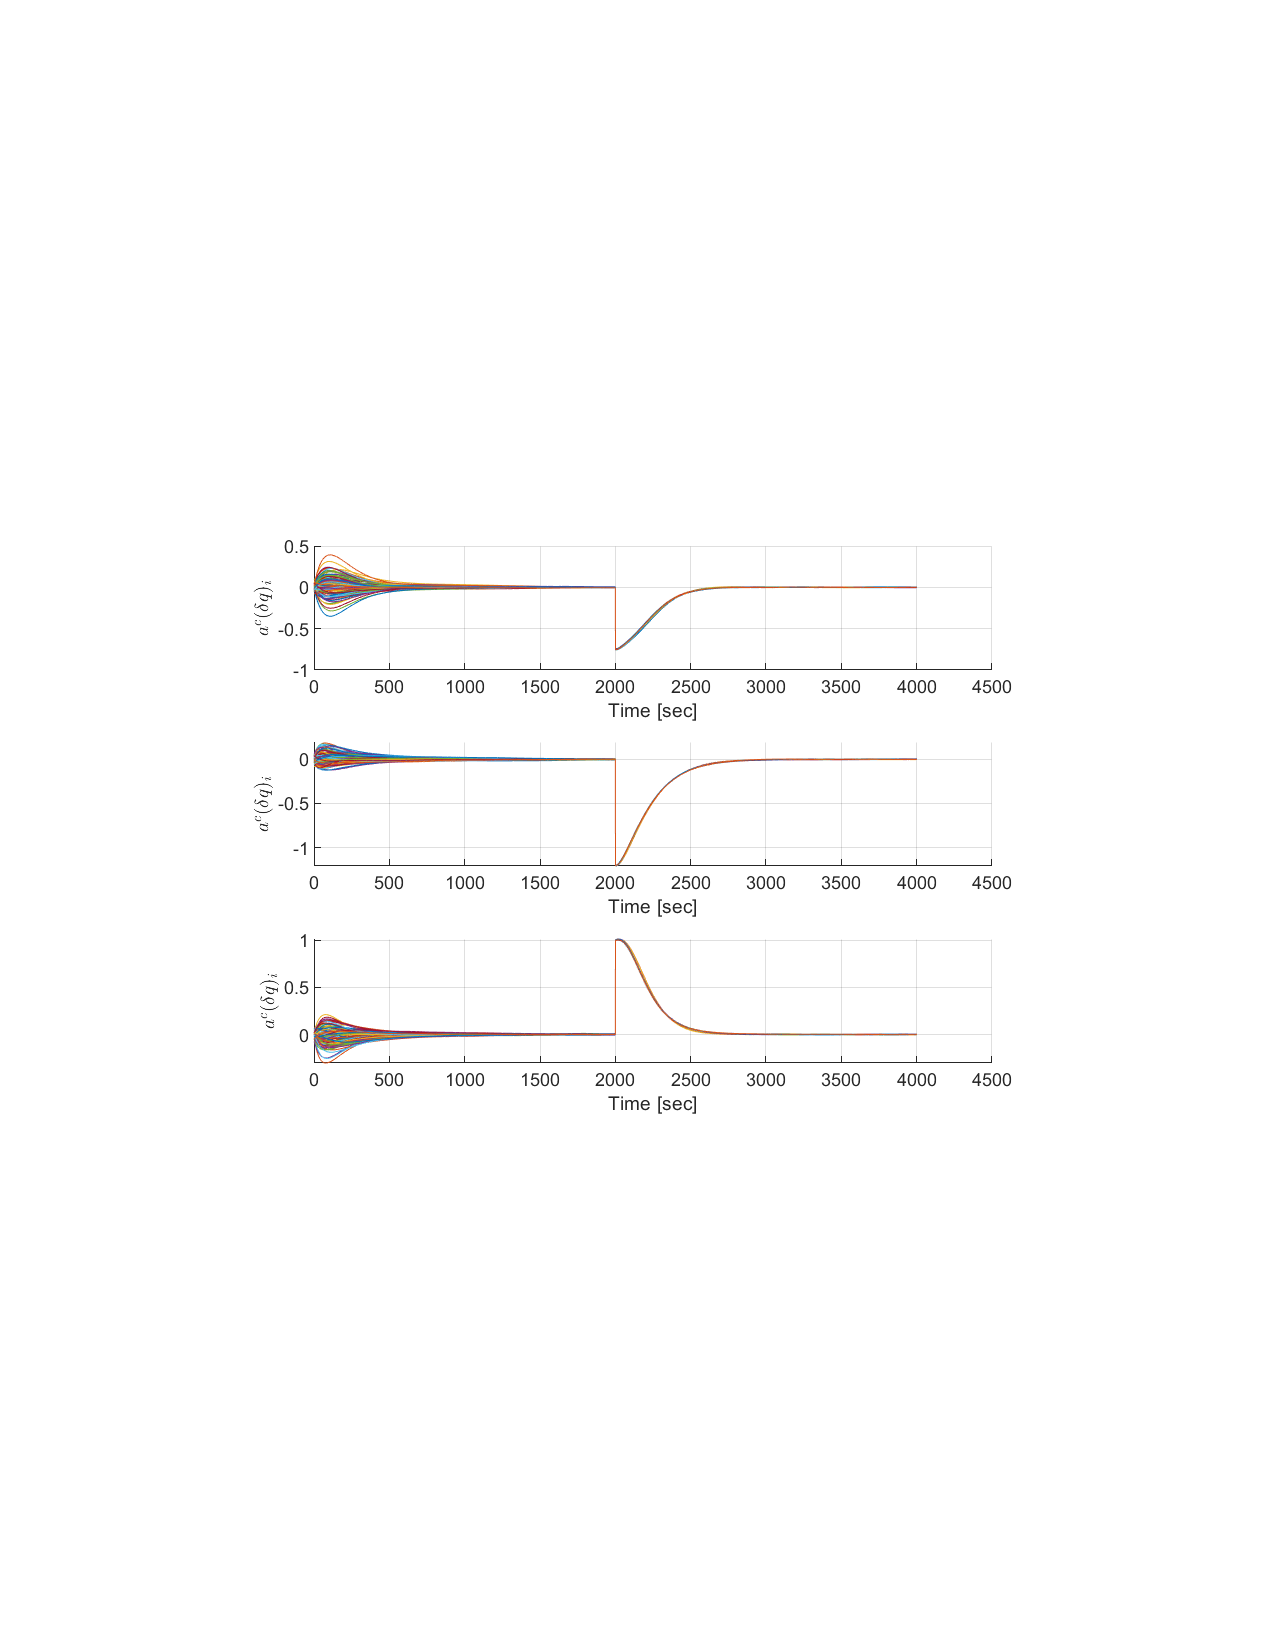
\includegraphics[width=\linewidth,trim={4cm, 8cm, 4cm, 8cm},clip]{figs/MC_quat_command_perf.pdf}
	\caption{The error in commanded inertial to body attitude for each MC run, expressed as a parameterization of the error quaternion. We begin with a constant rate maneuver, followed by a LVLH hold.}
	\label{fig:MC_quat_command_perf.pdf}
\end{figure}

\begin{figure}[!h]
	\centering
	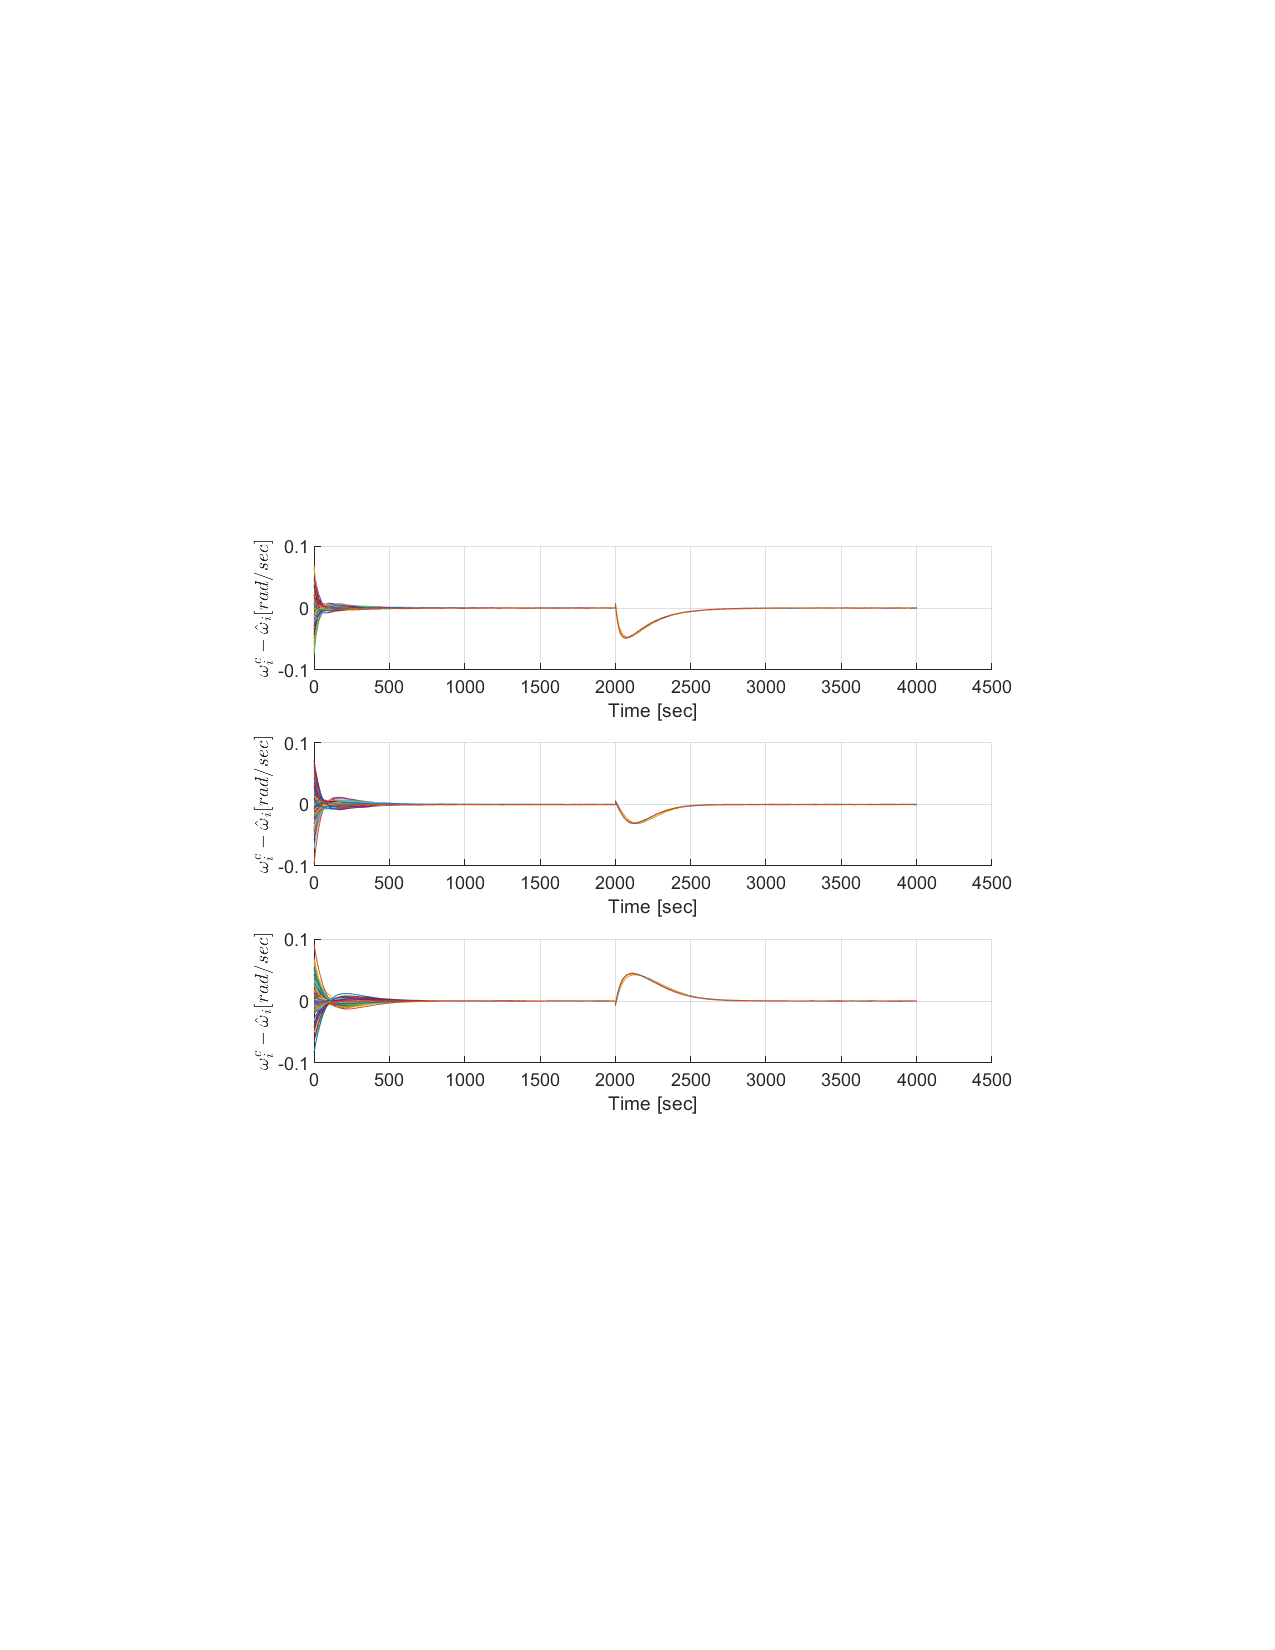
\includegraphics[width=\linewidth,trim={4cm, 8cm, 4cm, 8cm},clip]{figs/MC_rate_command_perf.pdf}
	\caption{The error in commanded body rate with respect to the inertial frame for each MC run. We begin with a constant rate maneuver, followed by a LVLH hold.}
	\label{fig:MC_rate_command_perf.pdf}
\end{figure}


\section{Actuators}

The station's actuators are CMGs which are exact replicas of those on the ISS. They have been upgraded to support infinite gimbal rotation rates. Our billionaire decided that electro-magnetic shielding on many critical components was unnecessary. This has a negative effect of introducing noise on the commanded torque for the CMGs. This is modeled as zero-mean Gaussian noise with covariance $10^{-6}\bm{I}_{3 \times 3}$.

The orientations of the CMGs are identical to those described in the first class midterm.

Figure \ref{fig:CMG_rates_1} shows CMG gimbal rates for one sample MC run.
\begin{figure}[!h]
	\centering
	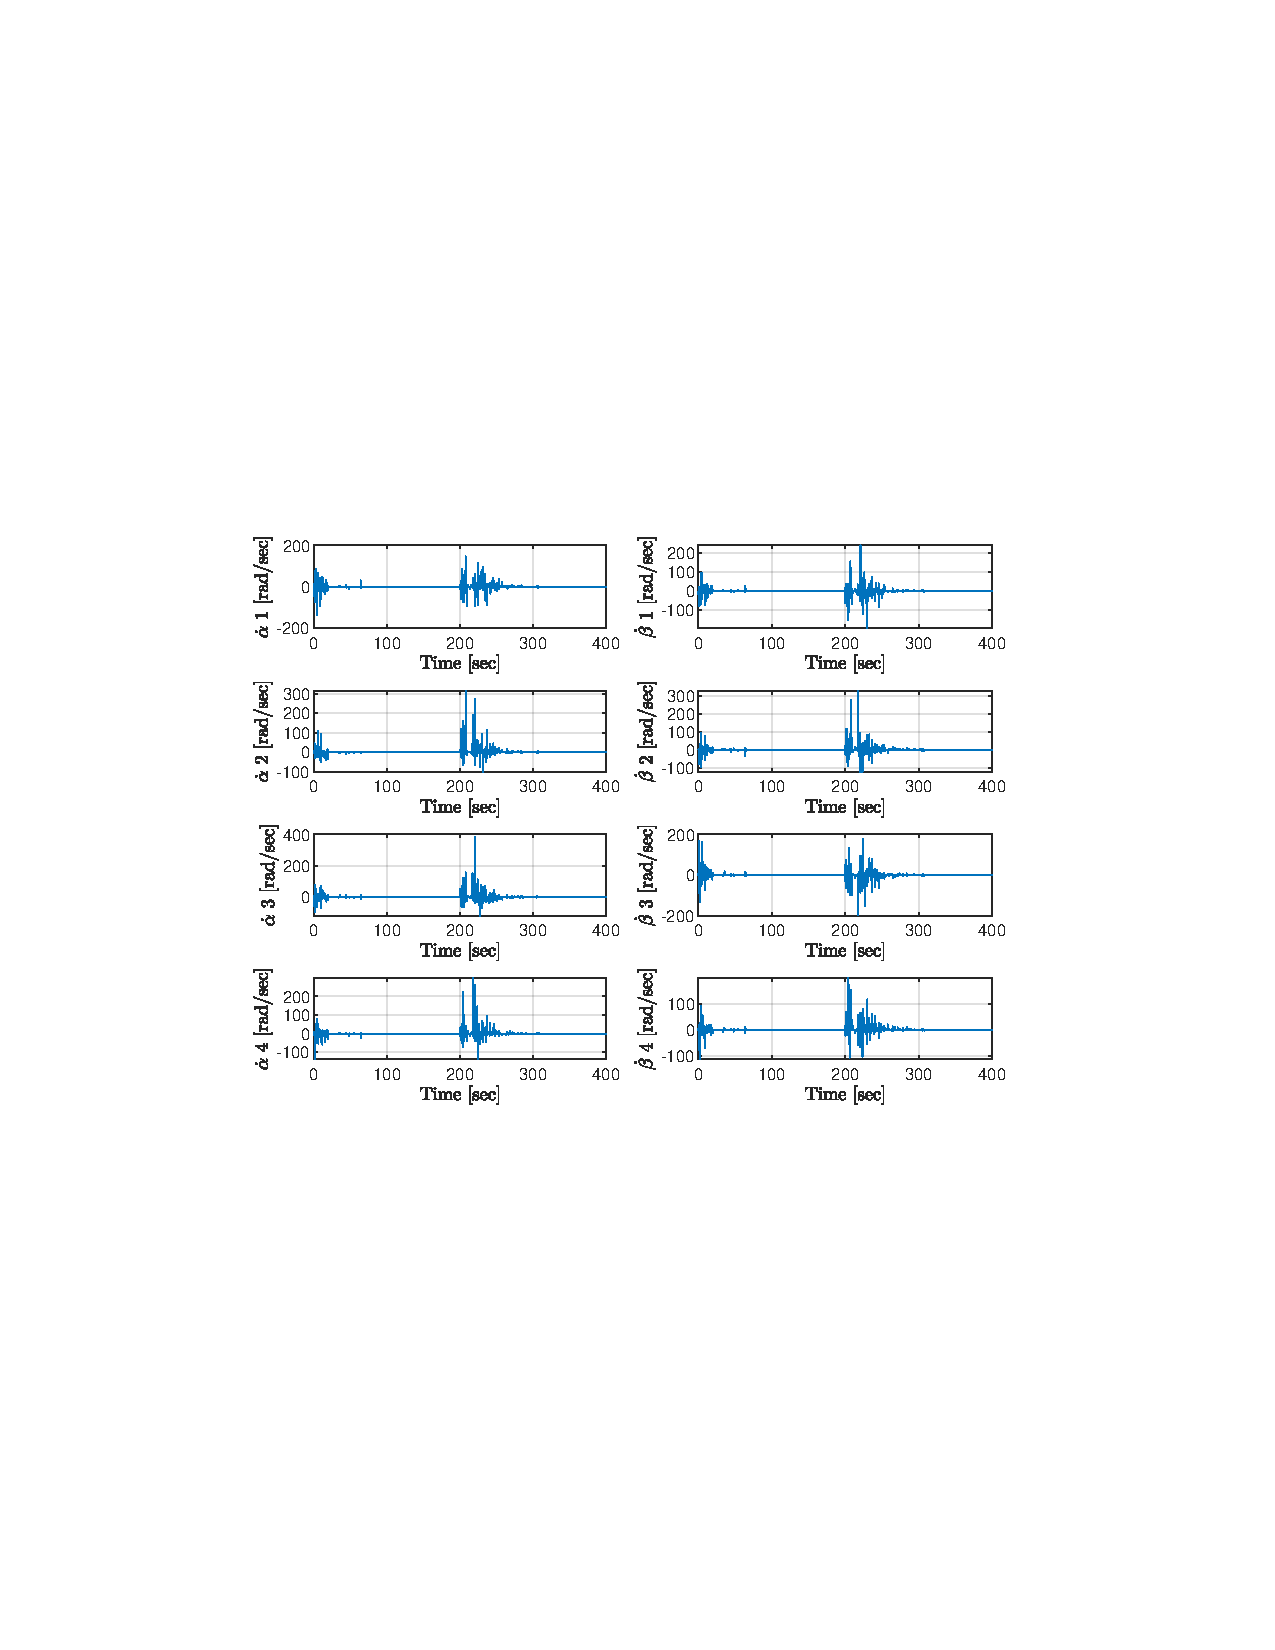
\includegraphics[width=\linewidth,trim={4cm, 8cm, 4cm, 8cm},clip]{figs/CMG_rates_1.pdf}
	\caption{The CMG gimbal rates for the first MC run.}
	\label{fig:CMG_rates_1}
\end{figure}

\section{Sensors}

The station's sensors include a gyroscope and star tracker. Neither sensor contains a bias and their true alignment is known. Both measurements occur at 10 Hz and are corrupted by zero-mean Gaussian noise. The noise covariance is $10^{-3}\bm{I}_{3 \times 3}$ for both sensors.

\section{MEKF}

The vehicle's true position and velocity are known. But it must use an MEKF to estimate its inertial to body attitude and angular rates. Both gyroscope and star tracker measurements are fused into the state during the update portion. The vehicle state is propagated using the torque command. We model process noise with covariance blkdiag\{$10^{-8}\bm{I}_{3 \times 3}$, $3.5\times10^{-11}\bm{I}_{3 \times 3}$\}. We implement underweighting by finding our Kalman Gain as $\bm{K} = \bm{PH}^T \left((1 + \beta)\bm{HPH}^T + \bm{R}\right)^{-1}$ where $\beta = 0.5$.

The initial state error is sampled from a zero-mean gaussian distribution with covariance blkdiag\{$10^{-3}\bm{I}_{3 \times 3}$, $10^{-4}\bm{I}_{3 \times 3}$\}.

Figures \ref{fig:MC_quat_est_perf.pdf} and \ref{fig:MC_rate_est_perf.pdf} show our MEKF performance. Our attitude representation is double the vector portion of the error quaternion. We see that our MEKF is unbiased, and slightly smug.

\begin{figure}[!h]
	\centering
	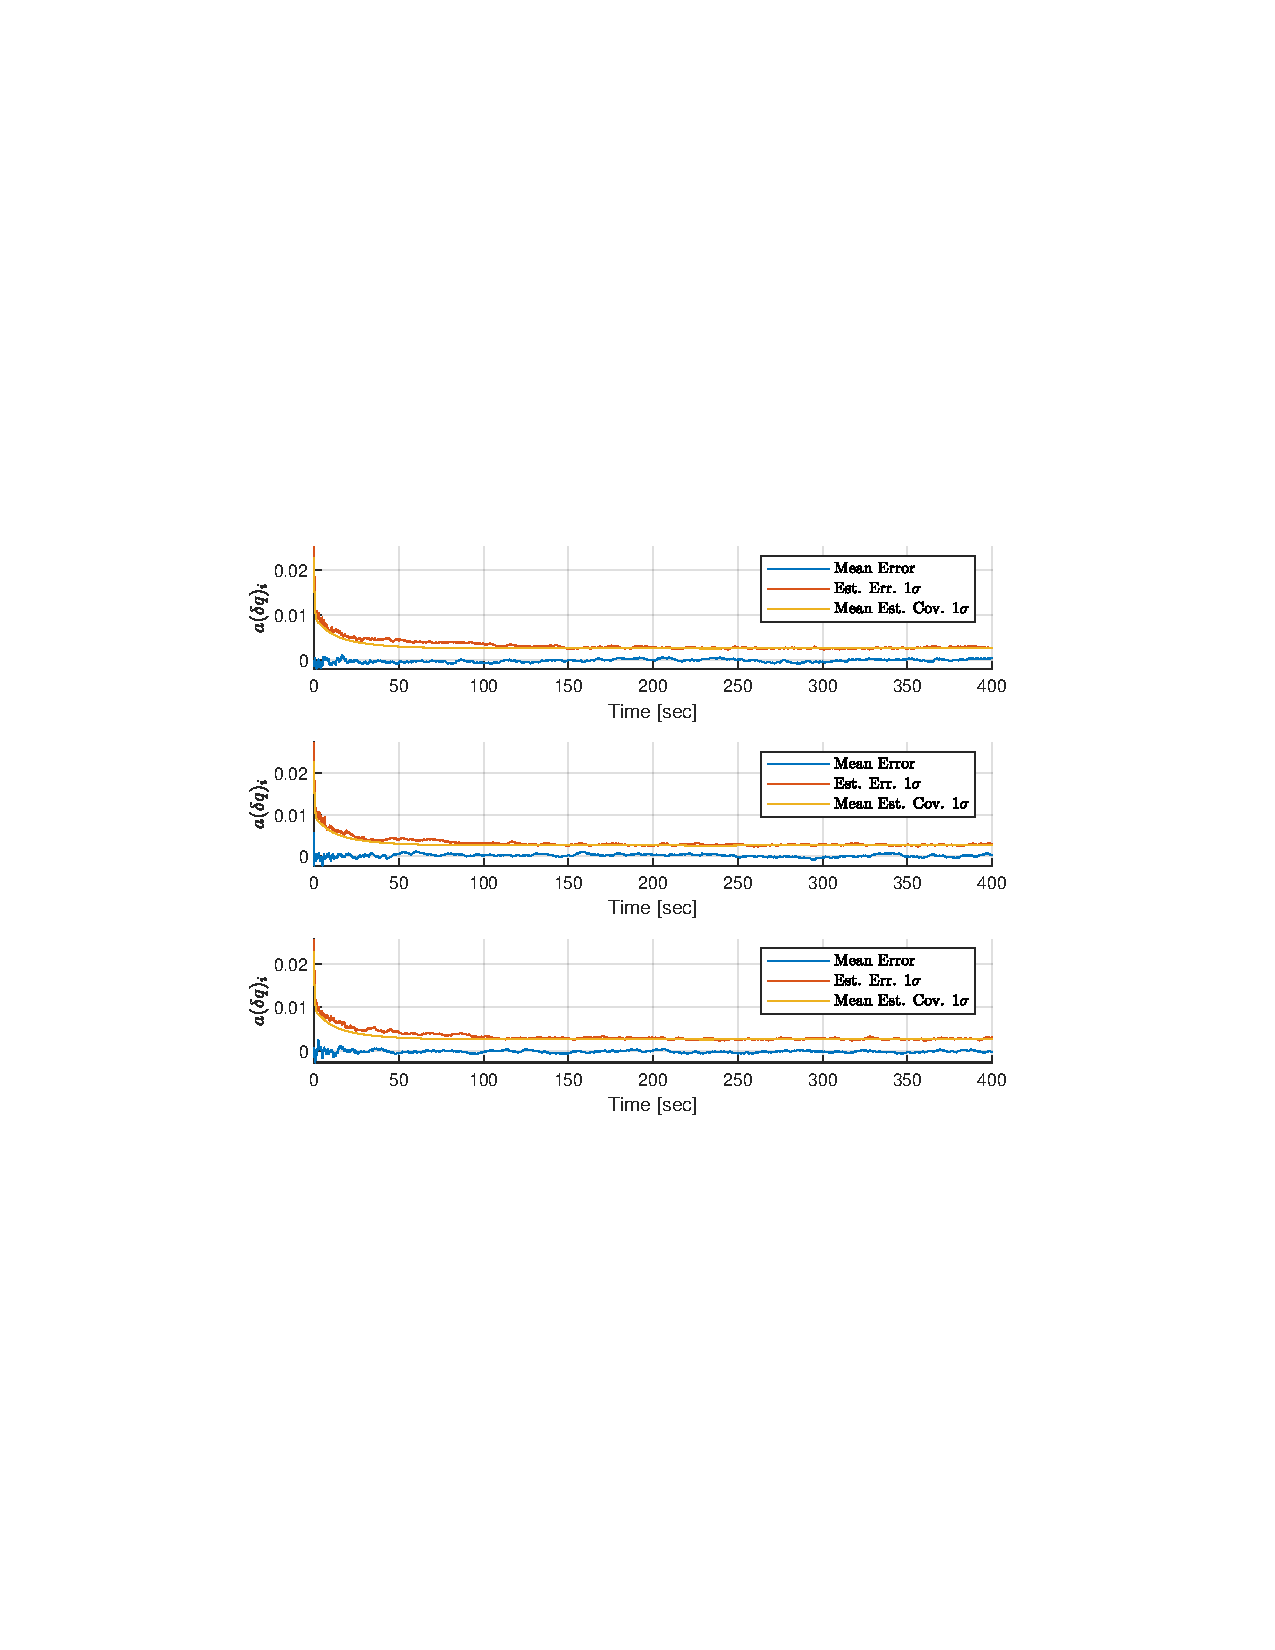
\includegraphics[width=\linewidth,trim={4cm, 8cm, 4cm, 8cm},clip]{figs/MC_quat_est_perf.pdf}
	\caption{The attitude estimation performance as shown by the average estimate error, sample error covariance, and average estimate covariance. We use an error parameterization which is double the vector component of the error quaternion.}
	\label{fig:MC_quat_est_perf.pdf}
\end{figure}

\begin{figure}[!h]
	\centering
	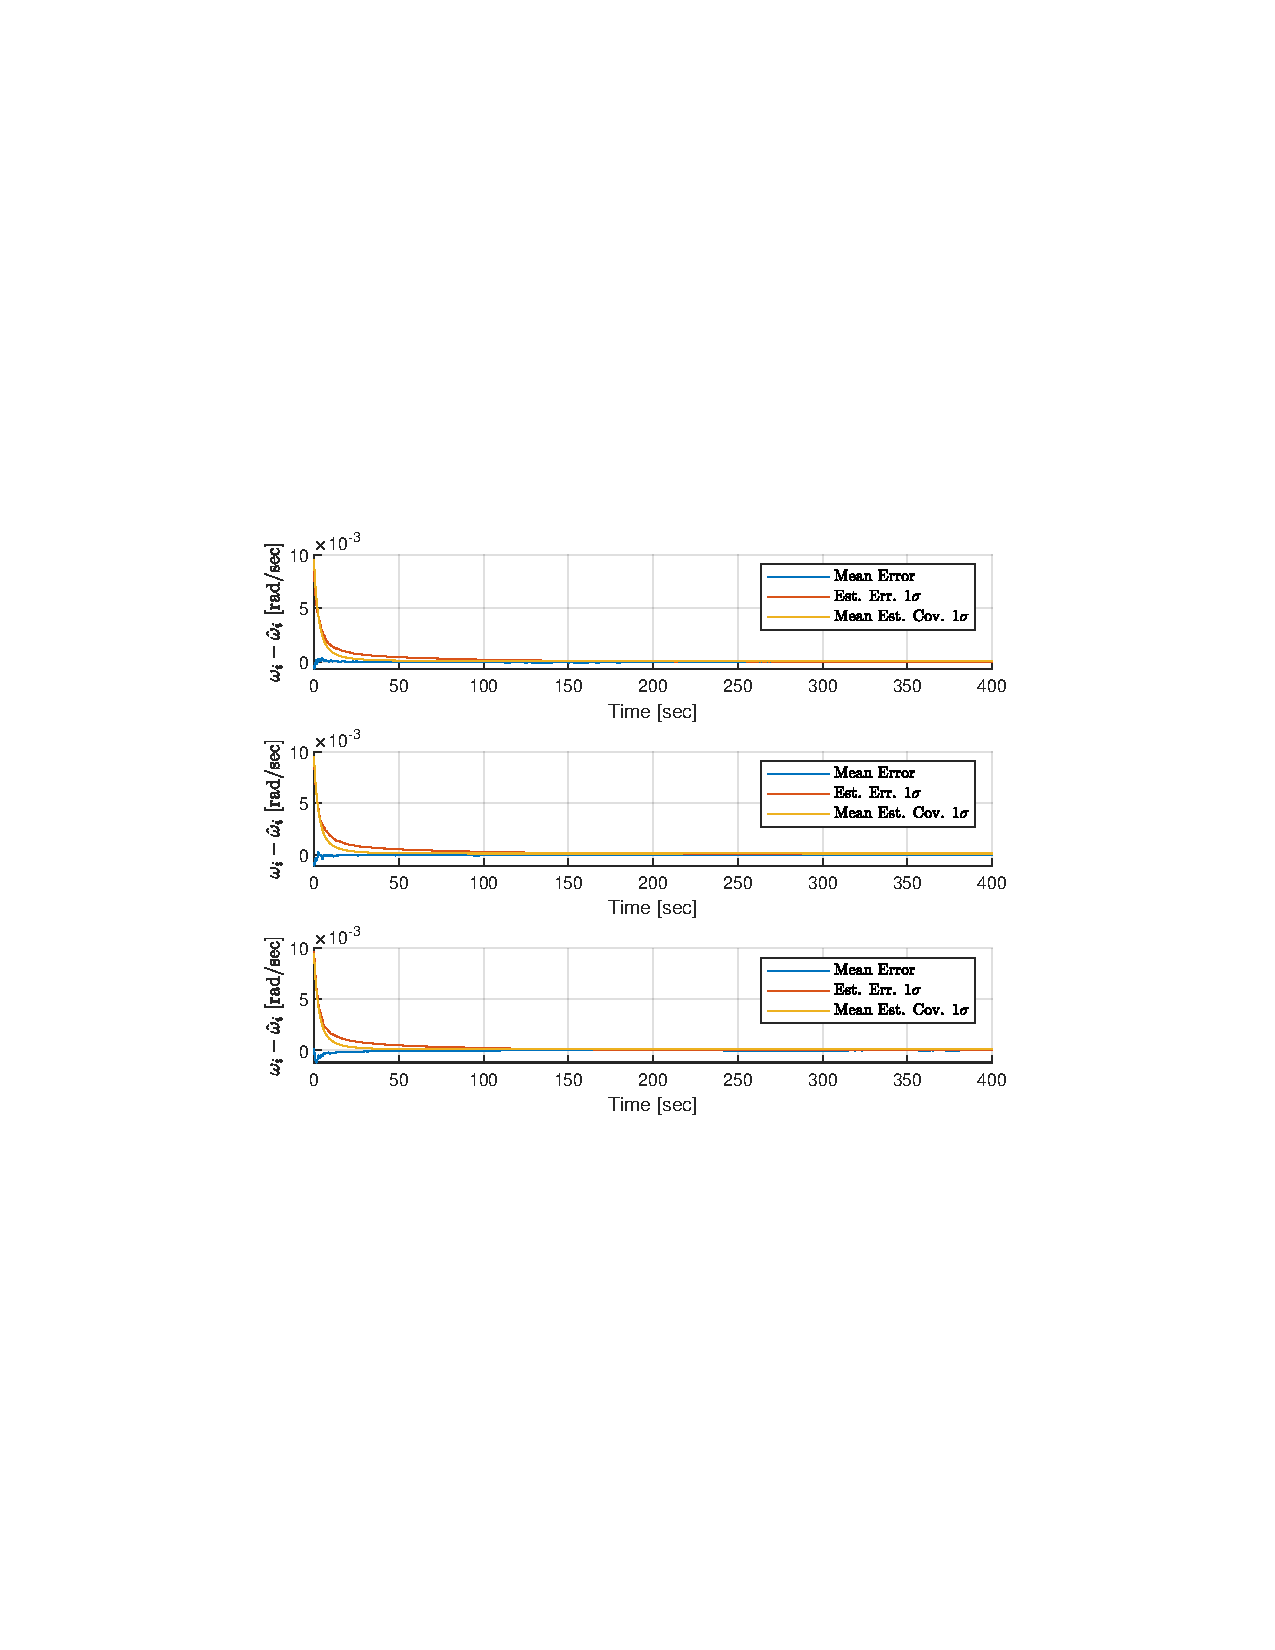
\includegraphics[width=\linewidth,trim={4cm, 8cm, 4cm, 8cm},clip]{figs/MC_rate_est_perf.pdf}
	\caption{The angular rate estimation performance as shown by the average estimate error, sample error covariance, and average estimate covariance.}
	\label{fig:MC_rate_est_perf.pdf}
\end{figure}


\section{Code}

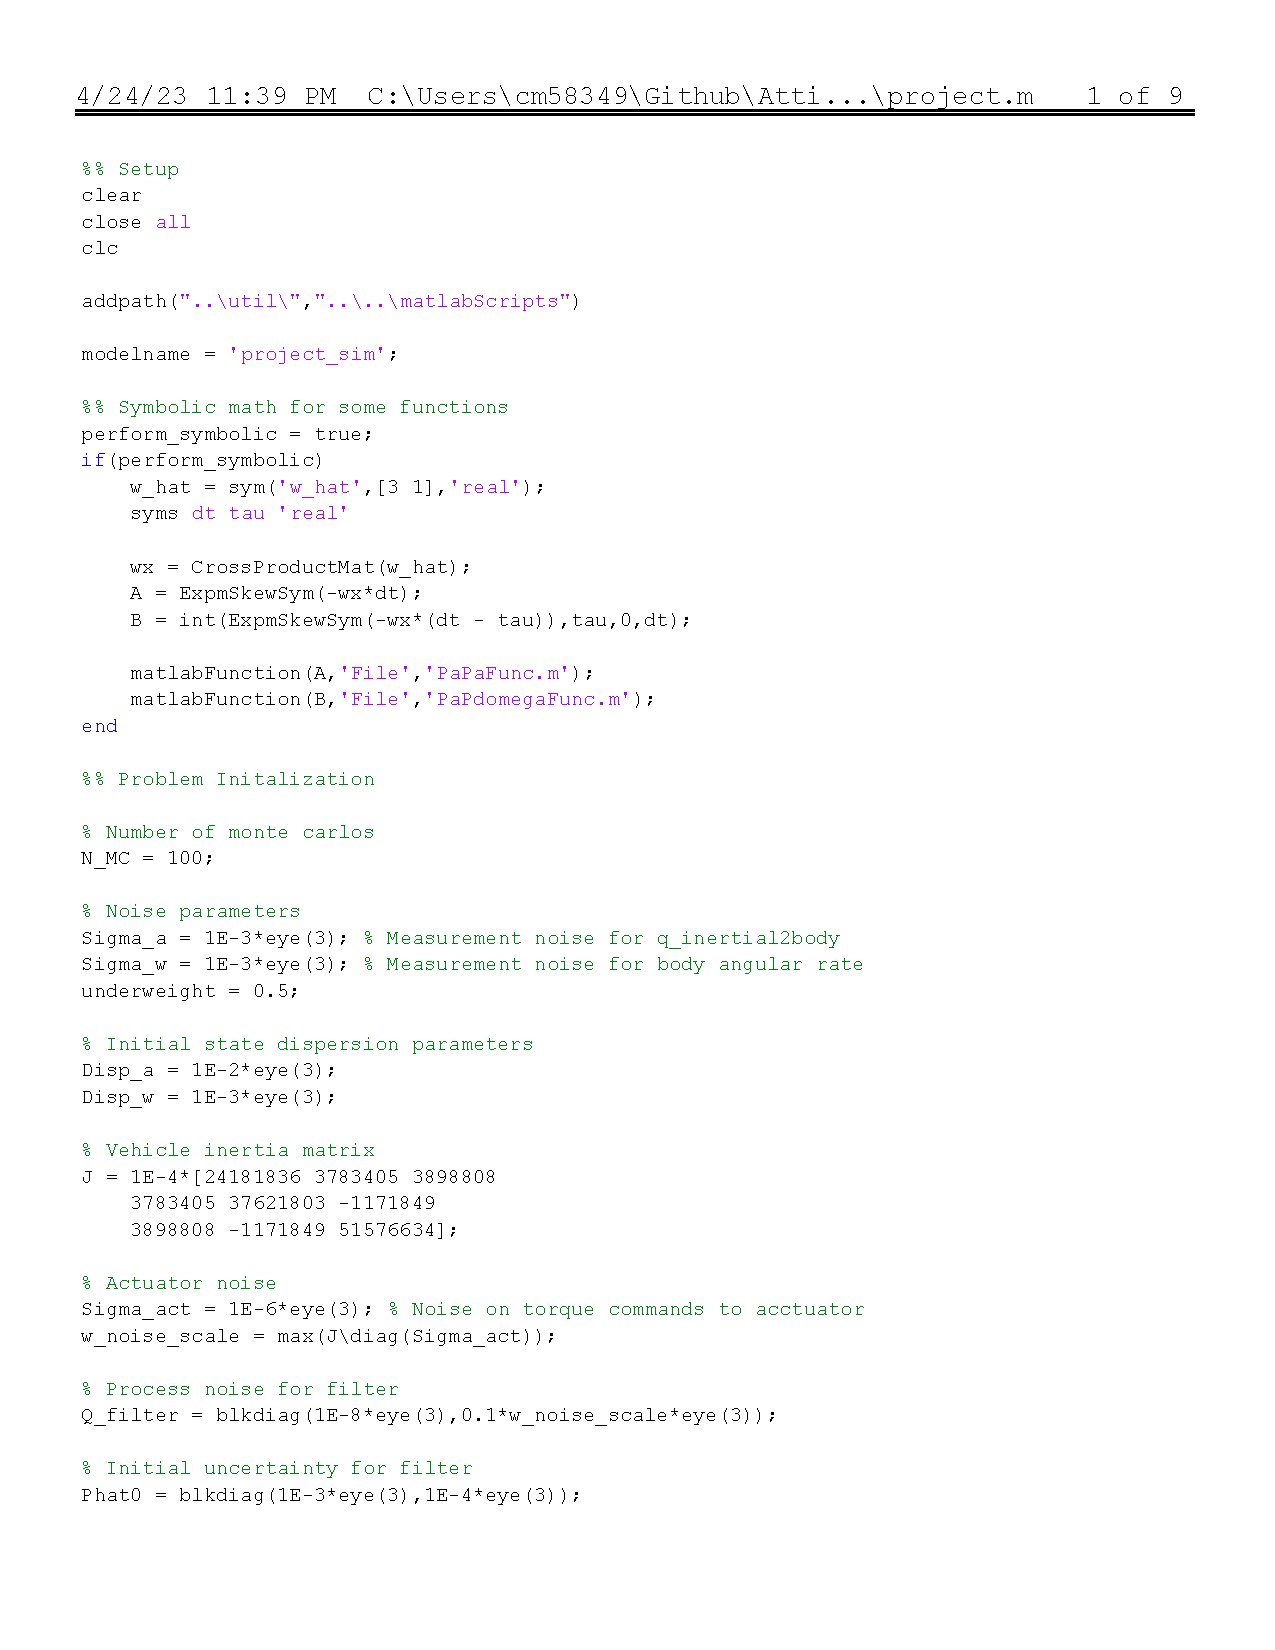
\includepdf[pages=-,pagecommand={},width=\textwidth]{code_main.pdf}
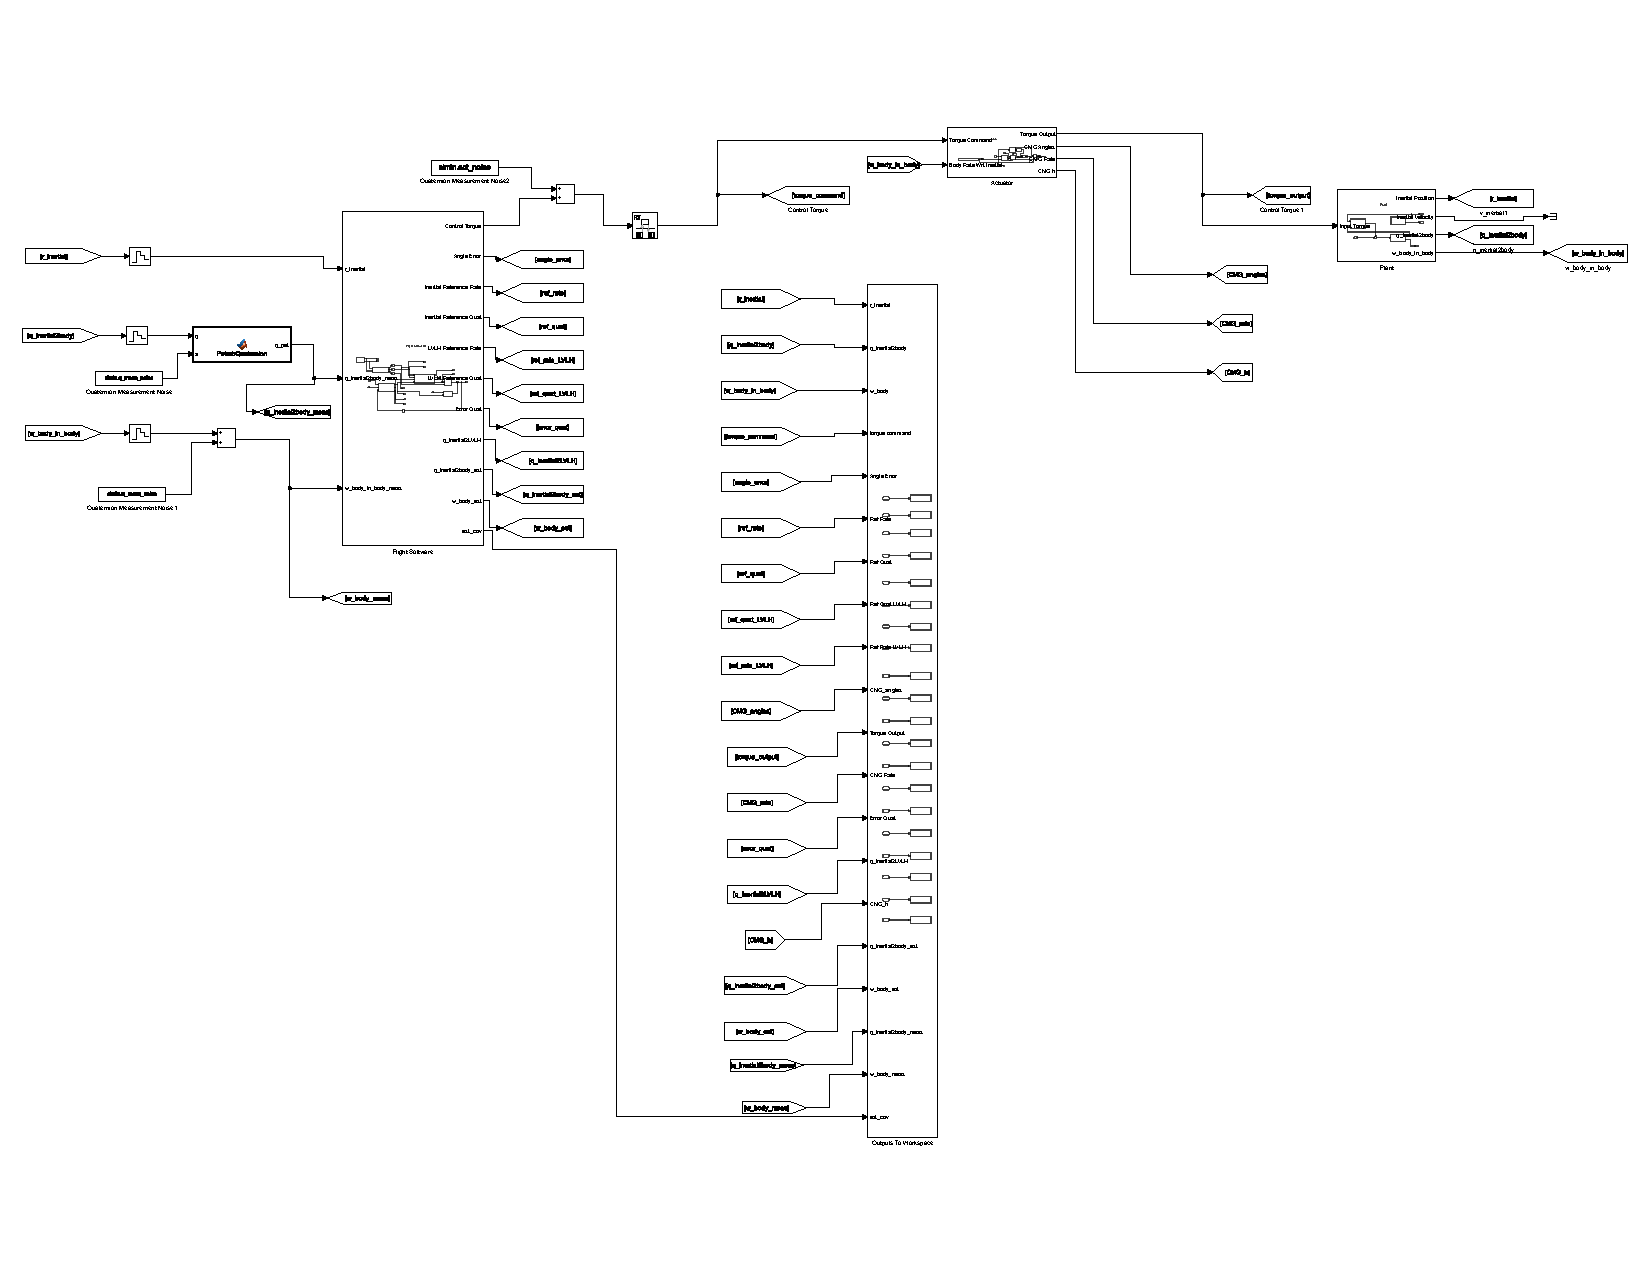
\includepdf[pages=-,pagecommand={},width=\textwidth]{code_doc.pdf}

\end{document}
